\section{Evaluation Suite Design}

The evaluation suite is designed to test whether high-level closed-loop
decision making with the LLM-centered closed-loop decision framework remains
effective as operational pressure increases. This requires more than evaluating
perception, planning, or replanning separately. Existing datasets and
evaluation settings only
partially cover the closed-loop rescue decision chain defined in Section~3. As
summarized in Table~\ref{tab:benchmark_comparison}, no existing setting jointly
evaluates the transition from aerial observation to task-zone construction,
resource-constrained mission planning, and runtime replanning. This comparison
concerns evaluation coverage rather than algorithmic performance.

% Required packages:
% \usepackage{booktabs}
% \usepackage{makecell}
% \usepackage{graphicx}

% Monochrome symbols are clearer and more appropriate for print publication.
\newcommand{\cmark}{\ensuremath{\bullet}}
\newcommand{\pmark}{\ensuremath{\circ}}
\newcommand{\xmark}{\textemdash}

\begin{table}[!t]
\centering
\caption{Coverage of evaluation capabilities in existing datasets, benchmarks,
and the evaluation suite used in this work.
\cmark indicates explicit coverage, \pmark indicates partial coverage, and \xmark indicates no explicit coverage.}
\label{tab:benchmark_comparison}
\footnotesize
\setlength{\tabcolsep}{1.5pt}
\renewcommand{\arraystretch}{1.08}
\begin{tabular}{
    @{}
    >{\raggedright\arraybackslash}p{0.32\columnwidth}
    *{4}{>{\centering\arraybackslash}p{0.14\columnwidth}}
    @{}}
\toprule
\textbf{Benchmark / dataset}
& \textbf{\makecell{Fire\\perc.}}
& \textbf{\makecell{Disaster\\sem.}}
& \textbf{\makecell{UAV\\constr.}}
& \textbf{\makecell{Runtime\\repl.}} \\
\midrule

DOTA~\cite{xia2018dota}
& \cmark & \xmark & \xmark & \xmark \\

VisDrone~\cite{zhu2022visdrone}
& \cmark & \xmark & \xmark & \xmark \\

UAVs-FFDB~\cite{mowla2024uavsffdb}
& \cmark & \cmark & \xmark & \xmark \\

FLAME~\cite{shamsoshoara2021flame}
& \cmark & \cmark & \xmark & \xmark \\

MS-FSDB~\cite{han2024msfsdb}
& \pmark & \cmark & \xmark & \xmark \\

WildFireVQA~\cite{habibpour2026wildfirevqa}
& \cmark & \cmark & \pmark & \xmark \\

RMASBench~\cite{kleiner2013rmasbench}
& \xmark & \cmark & \pmark & \pmark \\

CrisisBench~\cite{alam2021crisisbench}
& \xmark & \cmark & \xmark & \xmark \\

\midrule
\textbf{Our Evaluation Suite}
& \cmark & \cmark & \cmark & \cmark \\

\bottomrule
\end{tabular}
\end{table}


To close this gap, we instantiate the task model of Section~3 as a controlled,
real-UAV-informed evaluation suite in AirSim. The suite evaluates whether a
system can complete the full rescue loop within a single episode, from
fire-situation understanding to an executable plan and runtime replanning after
perturbations. The suite separately exposes task completion, execution quality,
and mission continuity, preventing high task completion from being interpreted
as uniformly effective execution under pressure. Its design combines three
complementary elements.

First, real-to-sim calibration constrains simulated platforms, sensing, and
mission conditions by the capabilities and safety limits of a real UAV. The
resulting evaluation episodes are therefore physically and operationally grounded rather
than arbitrarily configured. Second, difficulty stratification varies the
complexity of fire-point layouts, fleet-resource conditions, scheduling
interactions, and runtime perturbations while preserving a common task
definition. It enables controlled comparison of models and system mechanisms as
operational pressure increases. Third, mission-level metrics assess the
outcome of the complete rescue process from complementary operational
perspectives, rather than collapsing performance into a single score. The
following sections detail these three elements.

\begin{figure}[!t]
    \centering
    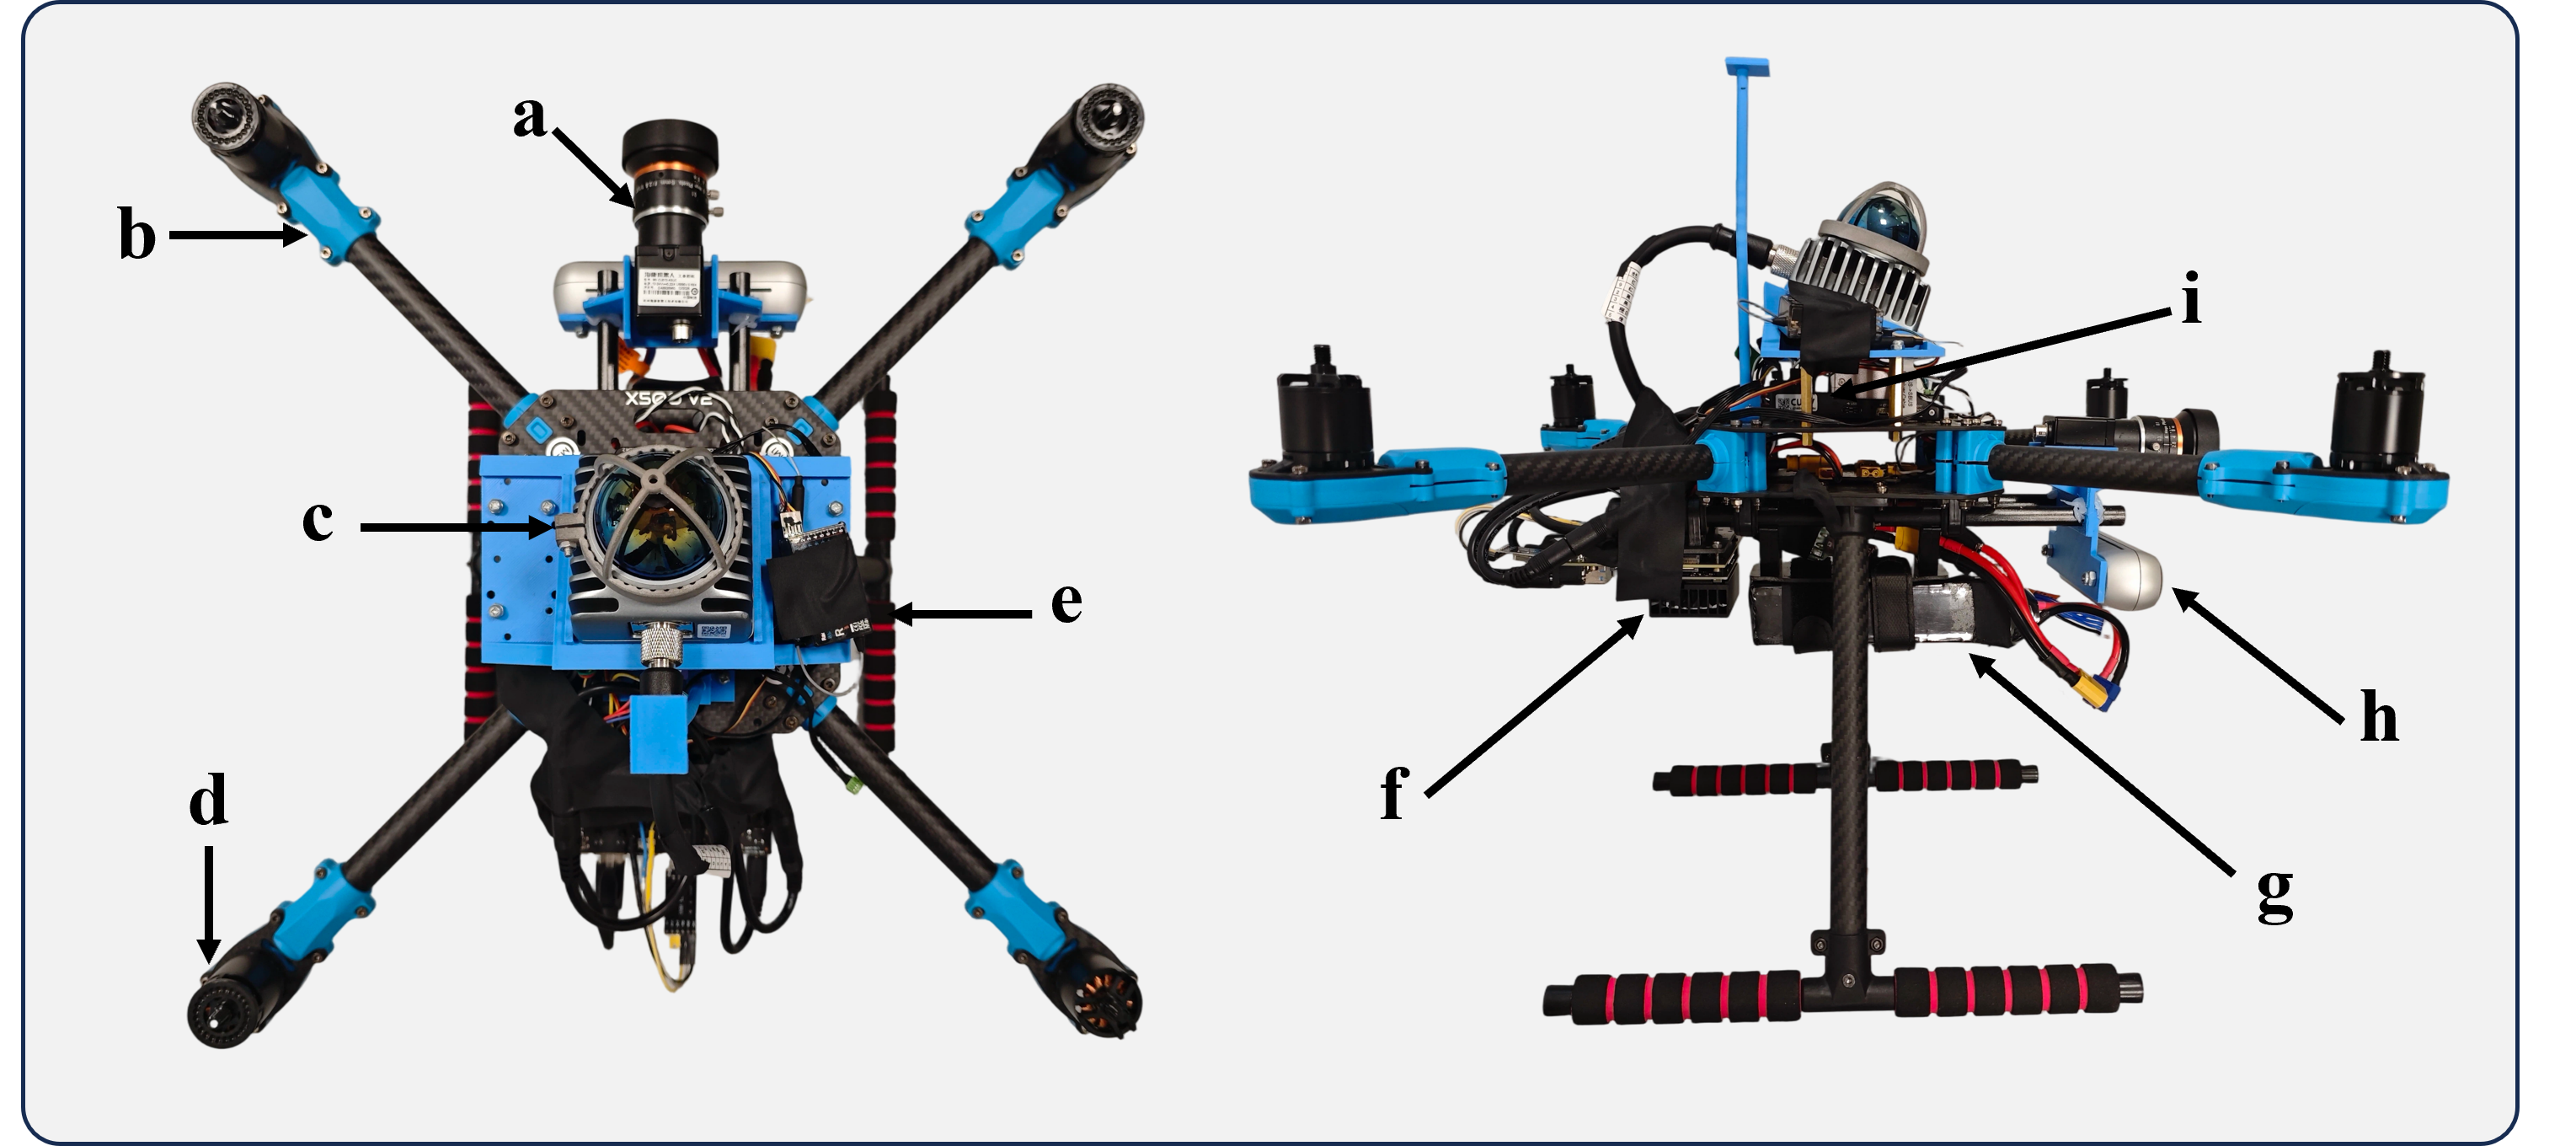
\includegraphics[width=\columnwidth]{figures/real-uav-platform.png}
    \caption{UAV platform and its main components: (a) LiDAR,
    (b) frame, (c) monocular camera, (d) motor, (e) receiver, 
    (f) onboard computer, (g) power supply, 
    (h) stereo camera, and (i) flight controller.}
    \label{fig:UAV-platform}
\end{figure}

\subsection{Real-to-Sim Calibration}
The first design property is realized through a co-design between the real UAV
platform and the AirSim simulation environment. As stated above, real UAV
parameters constrain every evaluation episode. Accordingly, the real platform defines the
engineering boundary of the rescue mission, while AirSim configures controllable
and repeatable evaluation episodes within that boundary. Rather than treating the two as
separate experimental settings, we use the real platform to define the feasible
set from which AirSim configures each simulated UAV and its environment.
For each UAV, the configured mission must satisfy
\begin{equation}
\begin{aligned}
\mathcal{E}_{\mathrm{UAV}}=\{&(h,v,m,e_{\mathrm{avail}},d)\mid\\
    &h\in \mathcal{H}_{\mathrm{safe}},\quad
      v\in \mathcal{V}_{\mathrm{safe}},\\
    &m\leq m_{\max},\quad
      e_{\mathrm{req}}+e_{\mathrm{res}}\leq e_{\mathrm{avail}},\\
    &d\leq d_{\mathrm{link}}\}.
\end{aligned}
\label{eq:uav-envelope}
\end{equation}
where $h$, $v$, $m$, $e_{\mathrm{avail}}$, and $d$ denote flight altitude,
velocity, payload mass, available energy, and distance to the coordination link. The safe altitude
and velocity ranges are specified by the operating policy. The payload and energy
bounds are grounded in the airframe, propulsion system, and battery; the energy
reserve enforces a safe return; and the link bound is determined by the deployed
communication configuration. Thus, the numerical bounds combine hardware
specifications, flight-safety policy, and deployment configuration. Any
configuration that violates
Eq.~\ref{eq:uav-envelope} is excluded before episode generation. The real UAV
platform is shown in Figure~\ref{fig:UAV-platform}, and its hardware
specifications are listed in Table~\ref{tab:real_uav_hardware}.

\input{tables/real-uav-hardware-specifications}

The virtual observation process is further fixed by the real camera geometry.
Under a nadir-view, locally planar-ground approximation, for altitude $h$,
horizontal field of view $\theta_{\mathrm{FOV}}$, and horizontal
resolution $N_x$, the image footprint and ground sampling distance are
\begin{equation}
W(h)=2h\tan\left(\frac{\theta_{\mathrm{FOV}}}{2}\right),\qquad
\mathrm{GSD}(h)=\frac{W(h)}{N_x}.
\label{eq:observation-geometry}
\end{equation}
Thus, the AirSim camera pose and the scale, density, and placement of fire
points are jointly constrained by what the real camera could observe, rather
than selected independently. Energy and payload limits likewise constrain route
length, task duration, and suppressible workload. Table~\ref{tab:real_to_sim_calibration}
records these calibration rules and the resulting simulation settings.

\input{tables/airsim-real-to-sim-calibration}

These calibrated bounds provide the common operational basis on which the
difficulty levels are constructed.

\subsection{Difficulty Stratification}
The second design property is that each evaluation episode is purpose-built
rather than randomly sampled.
Each episode instantiates the task variables defined in Section~3 through three
controlled dimensions: fleet and resource conditions, fire-point layouts, and,
where applicable, runtime perturbations. Their combinations define four
stress-testing difficulty levels in Table~\ref{tab:scenario-controls}. Each
difficulty level is instantiated by a fixed set of 20 evaluation episodes,
yielding 80 episodes in total.

The four levels form a staged operational-pressure axis rather than four
unrelated scenario groups. The simple and normal levels test fire-situation
understanding and resource-constrained mission planning under progressively
tighter initial conditions. The hard and expert levels retain these pressures
while adding runtime perturbations and stronger scheduling interactions. This
progression makes episode difficulty useful not only for measuring end-to-end
degradation, but also for identifying when Validation, Memory, and Runtime
Replanning become consequential.

\input{tables/scenario-difficulty-controls}

The fleet and resource conditions in every evaluation episode are constrained by the
real-to-sim calibration in Section~4.1. In particular, each simulated UAV must
satisfy the feasible operating envelope in Eq.~\ref{eq:uav-envelope}, and its
imaging, energy, payload, and communication settings follow
Table~\ref{tab:real_to_sim_calibration}. Difficulty is therefore varied only
within the engineering and operational limits established for the real platform.

The fire-point configurations of all episodes are pre-specified rather than
randomly generated. These configurations control the scene structure
and the spatial arrangement and number of fire points per task zone across
difficulty levels.
Figure~\ref{fig:difficulty-scene-examples} provides representative scenes from
the four difficulty levels, and Figure~\ref{fig:fire-point-count-distribution} summarizes
the distribution of fire-point counts per task zone within each difficulty level. Together,
they illustrate the scene layouts and task-zone-level fire-point distributions
used to instantiate the four difficulty levels.

\begin{figure*}[!t]
    \centering
    \includegraphics[width=1\textwidth]{figures/difficulty-level-fire-scenes.png}
    \caption{Representative fire scenes from the four difficulty levels.
    In each example, \textit{Origin image} denotes the original aerial image,
    and \textit{Perception result} denotes the output generated by the Vision
    Analysis module, which uses Gemini~3.1 Pro as its foundation model.}
    \label{fig:difficulty-scene-examples}
\end{figure*}

\begin{figure}[!t]
    \centering
    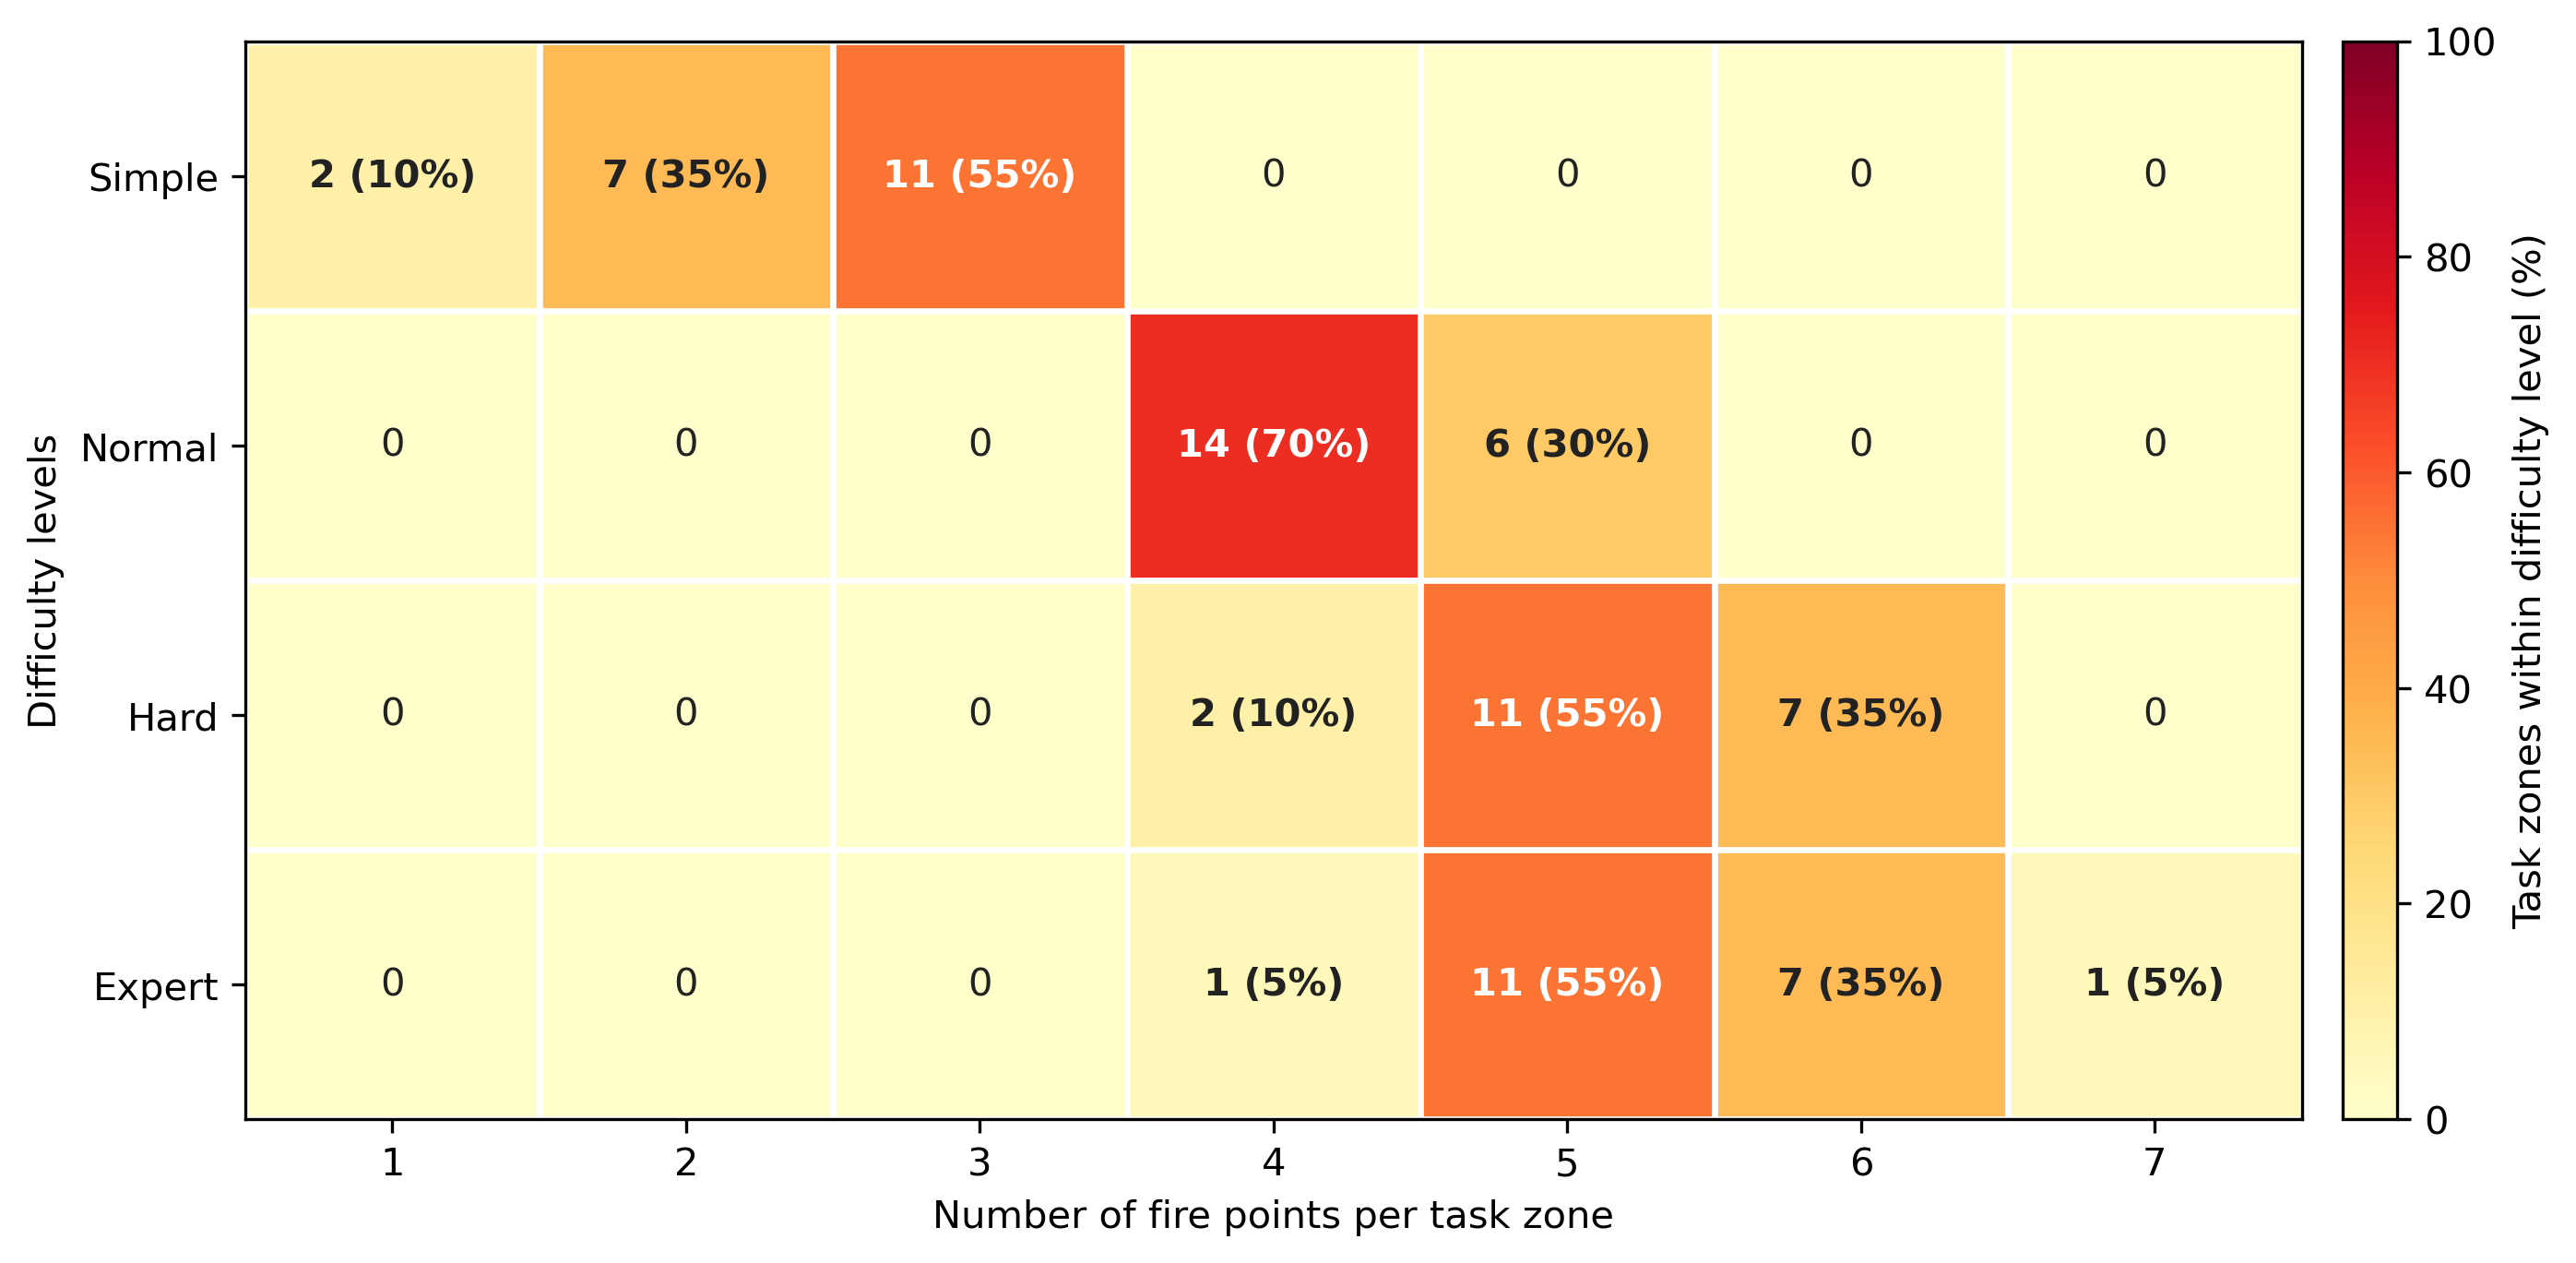
\includegraphics[width=\columnwidth]{figures/task-zone-fire-point-distribution.png}
    \caption{Distribution of fire-point counts per task zone across difficulty
    levels.}
    \label{fig:fire-point-count-distribution}
\end{figure}

The third controlled dimension introduces runtime perturbations after mission
execution has begun. Unlike the preceding two dimensions, which specify the
initial fleet state and fire scene, these events modify the operational state
or mission constraints faced by an active plan. For this evaluation suite, we
construct our own runtime perturbation library comprising five families: fire evolution (30\%),
UAV-state failure (24\%), zone evolution (19\%), scheduling constraint (14\%),
and resource failure (13\%). As shown in
Figure~\ref{fig:runtime-perturbation-distribution}(a), each family contains
concrete event types, such as new fire sources and fire spreading, positioning,
sensor, and communication failures, boundary changes and affected-area
expansion, human commands and priority changes, and load exhaustion and energy
shortage.

Runtime perturbations are enabled only in the hard and expert levels and are
placed at predefined points in each episode so that replanning behavior can be
evaluated under repeatable conditions. During suite construction, events are
drawn once from the library according to the configured sampling distribution
and then fixed within the evaluation episodes.
Hard episodes contain a small number of temporally separated perturbations,
whereas expert episodes contain more frequent perturbations that may occur
concurrently or in succession and impose stronger communication and global
scheduling pressure. Figure~\ref{fig:runtime-perturbation-distribution}(b)
shows the resulting draws by perturbation family: expert episodes contain more
events in every family, while preserving coverage of all five families.

\begin{figure*}[!t]
    \centering
    \subfloat[Runtime perturbation library.]{%
        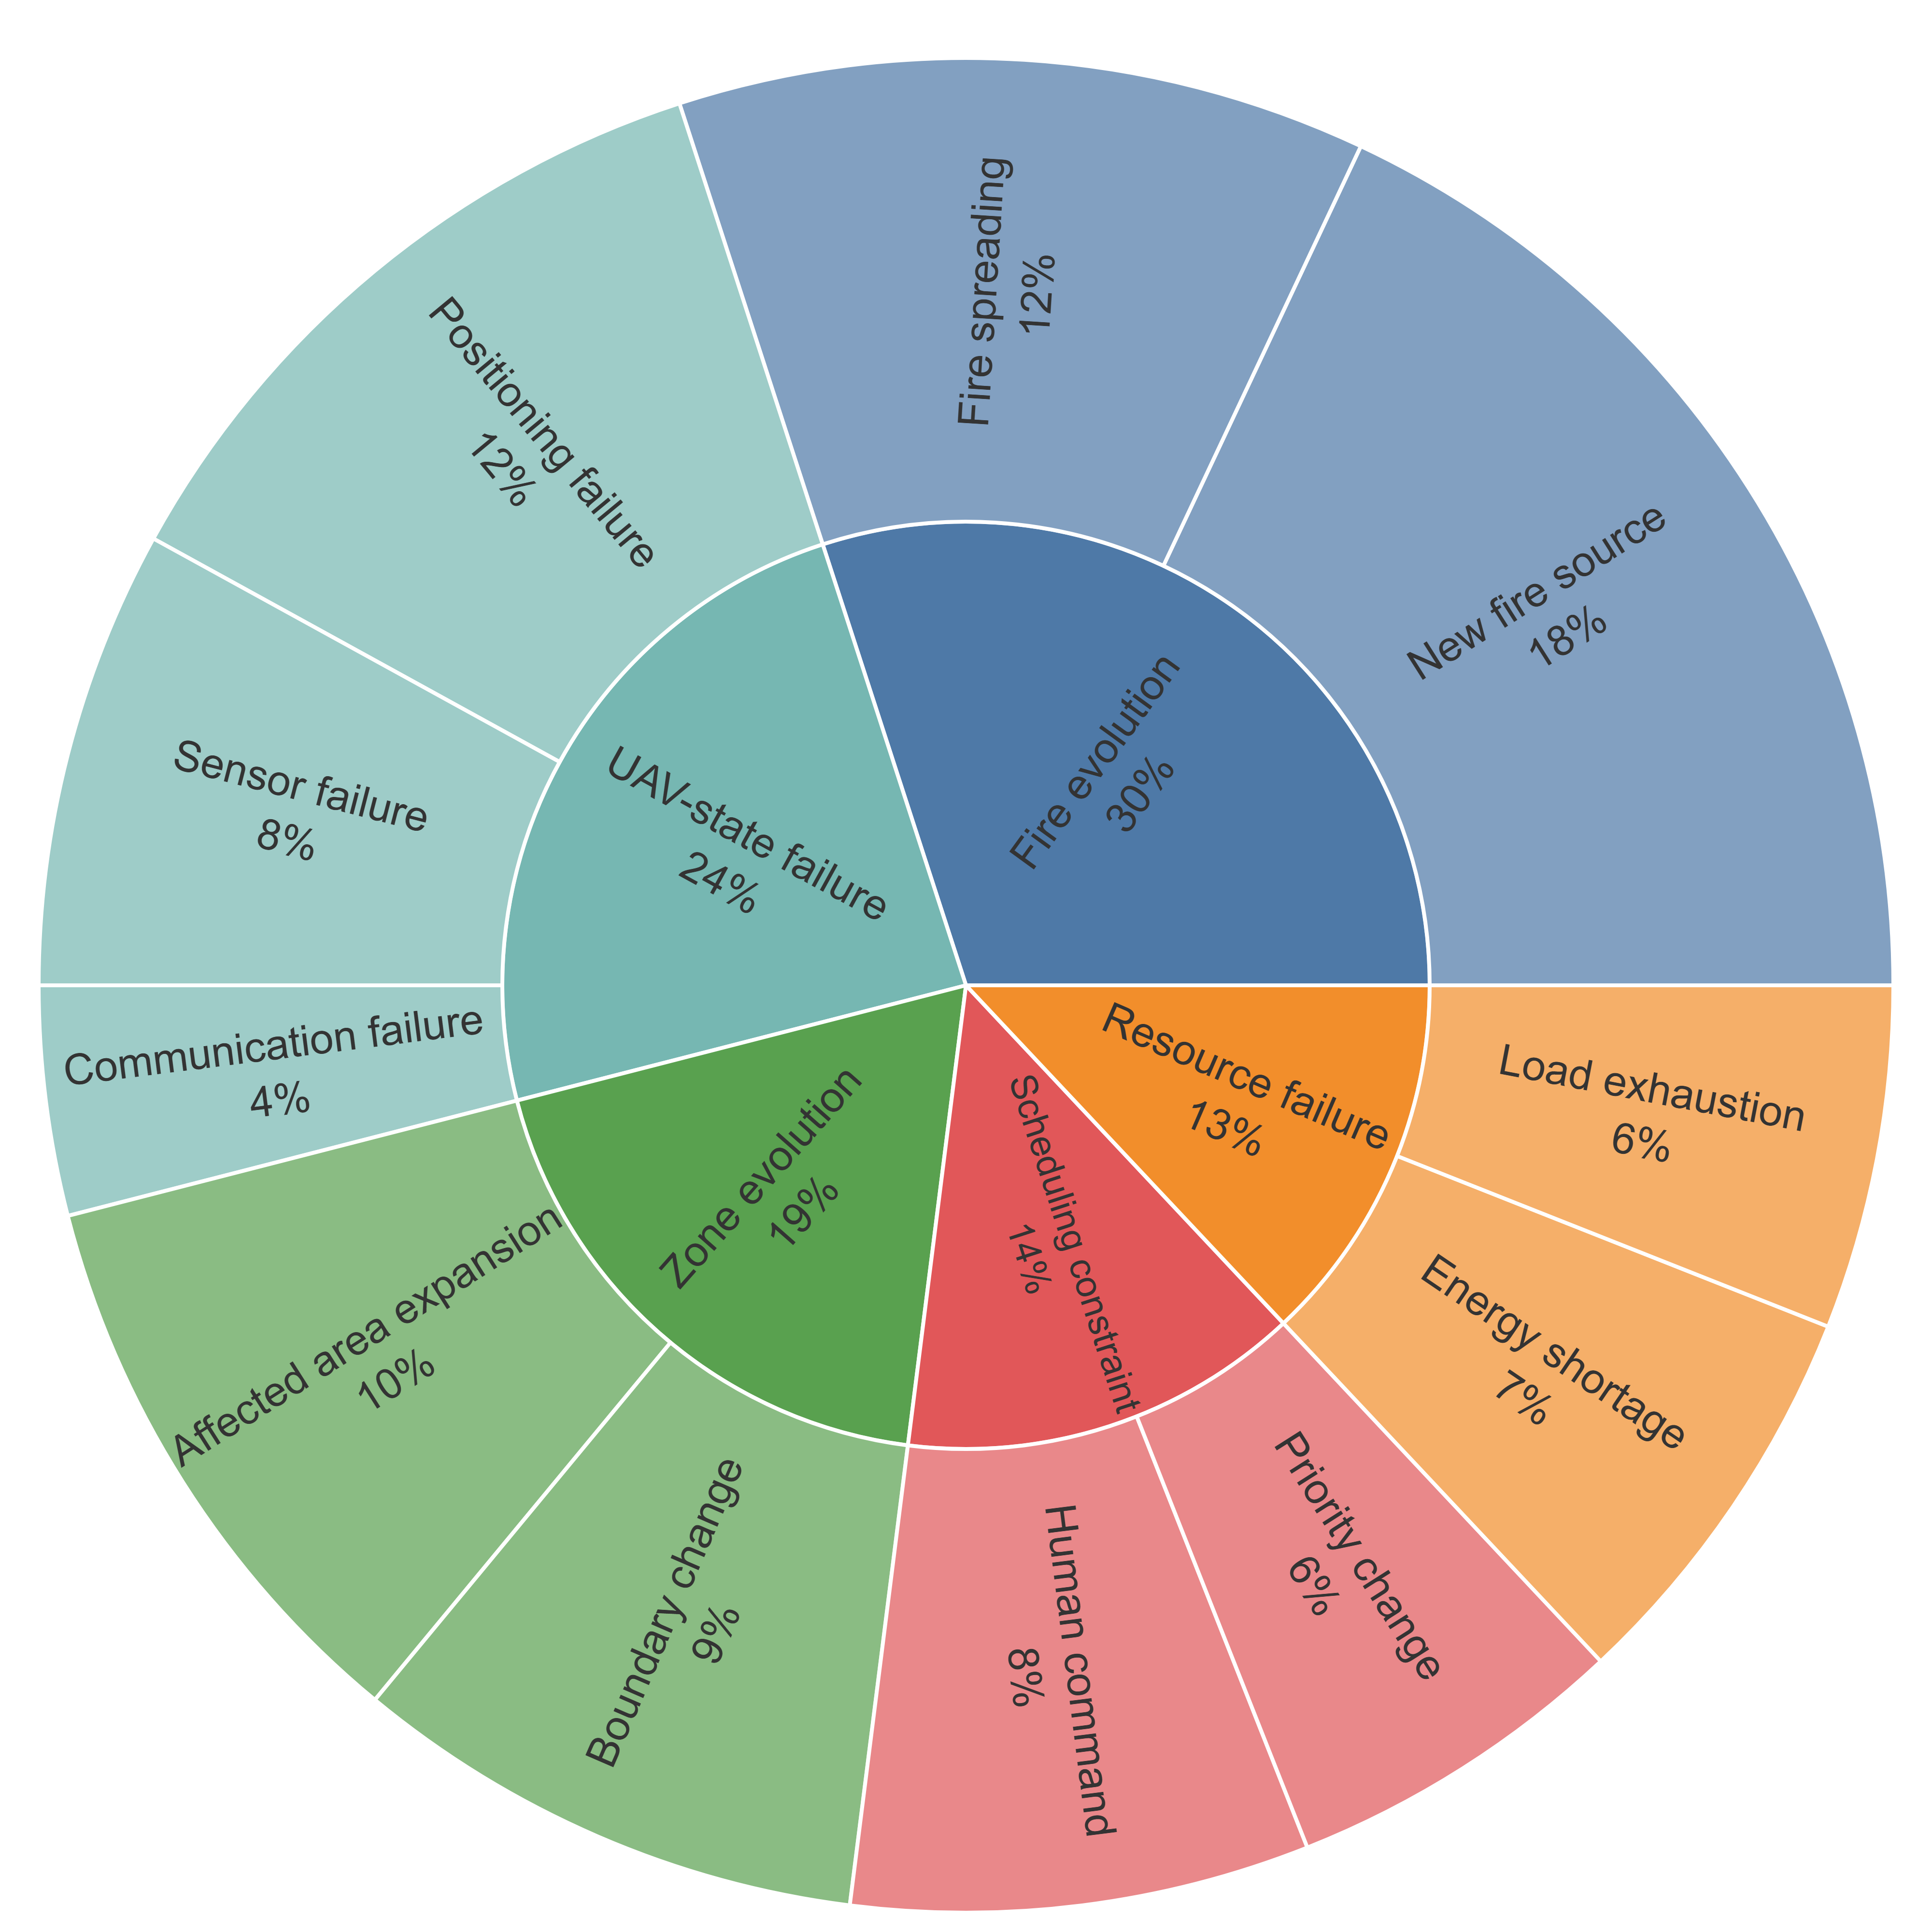
\includegraphics[width=0.485\textwidth]{figures/runtime-perturbation-library.png}}\hfill
    \subfloat[Distribution of perturbations in hard and expert levels.]{%
        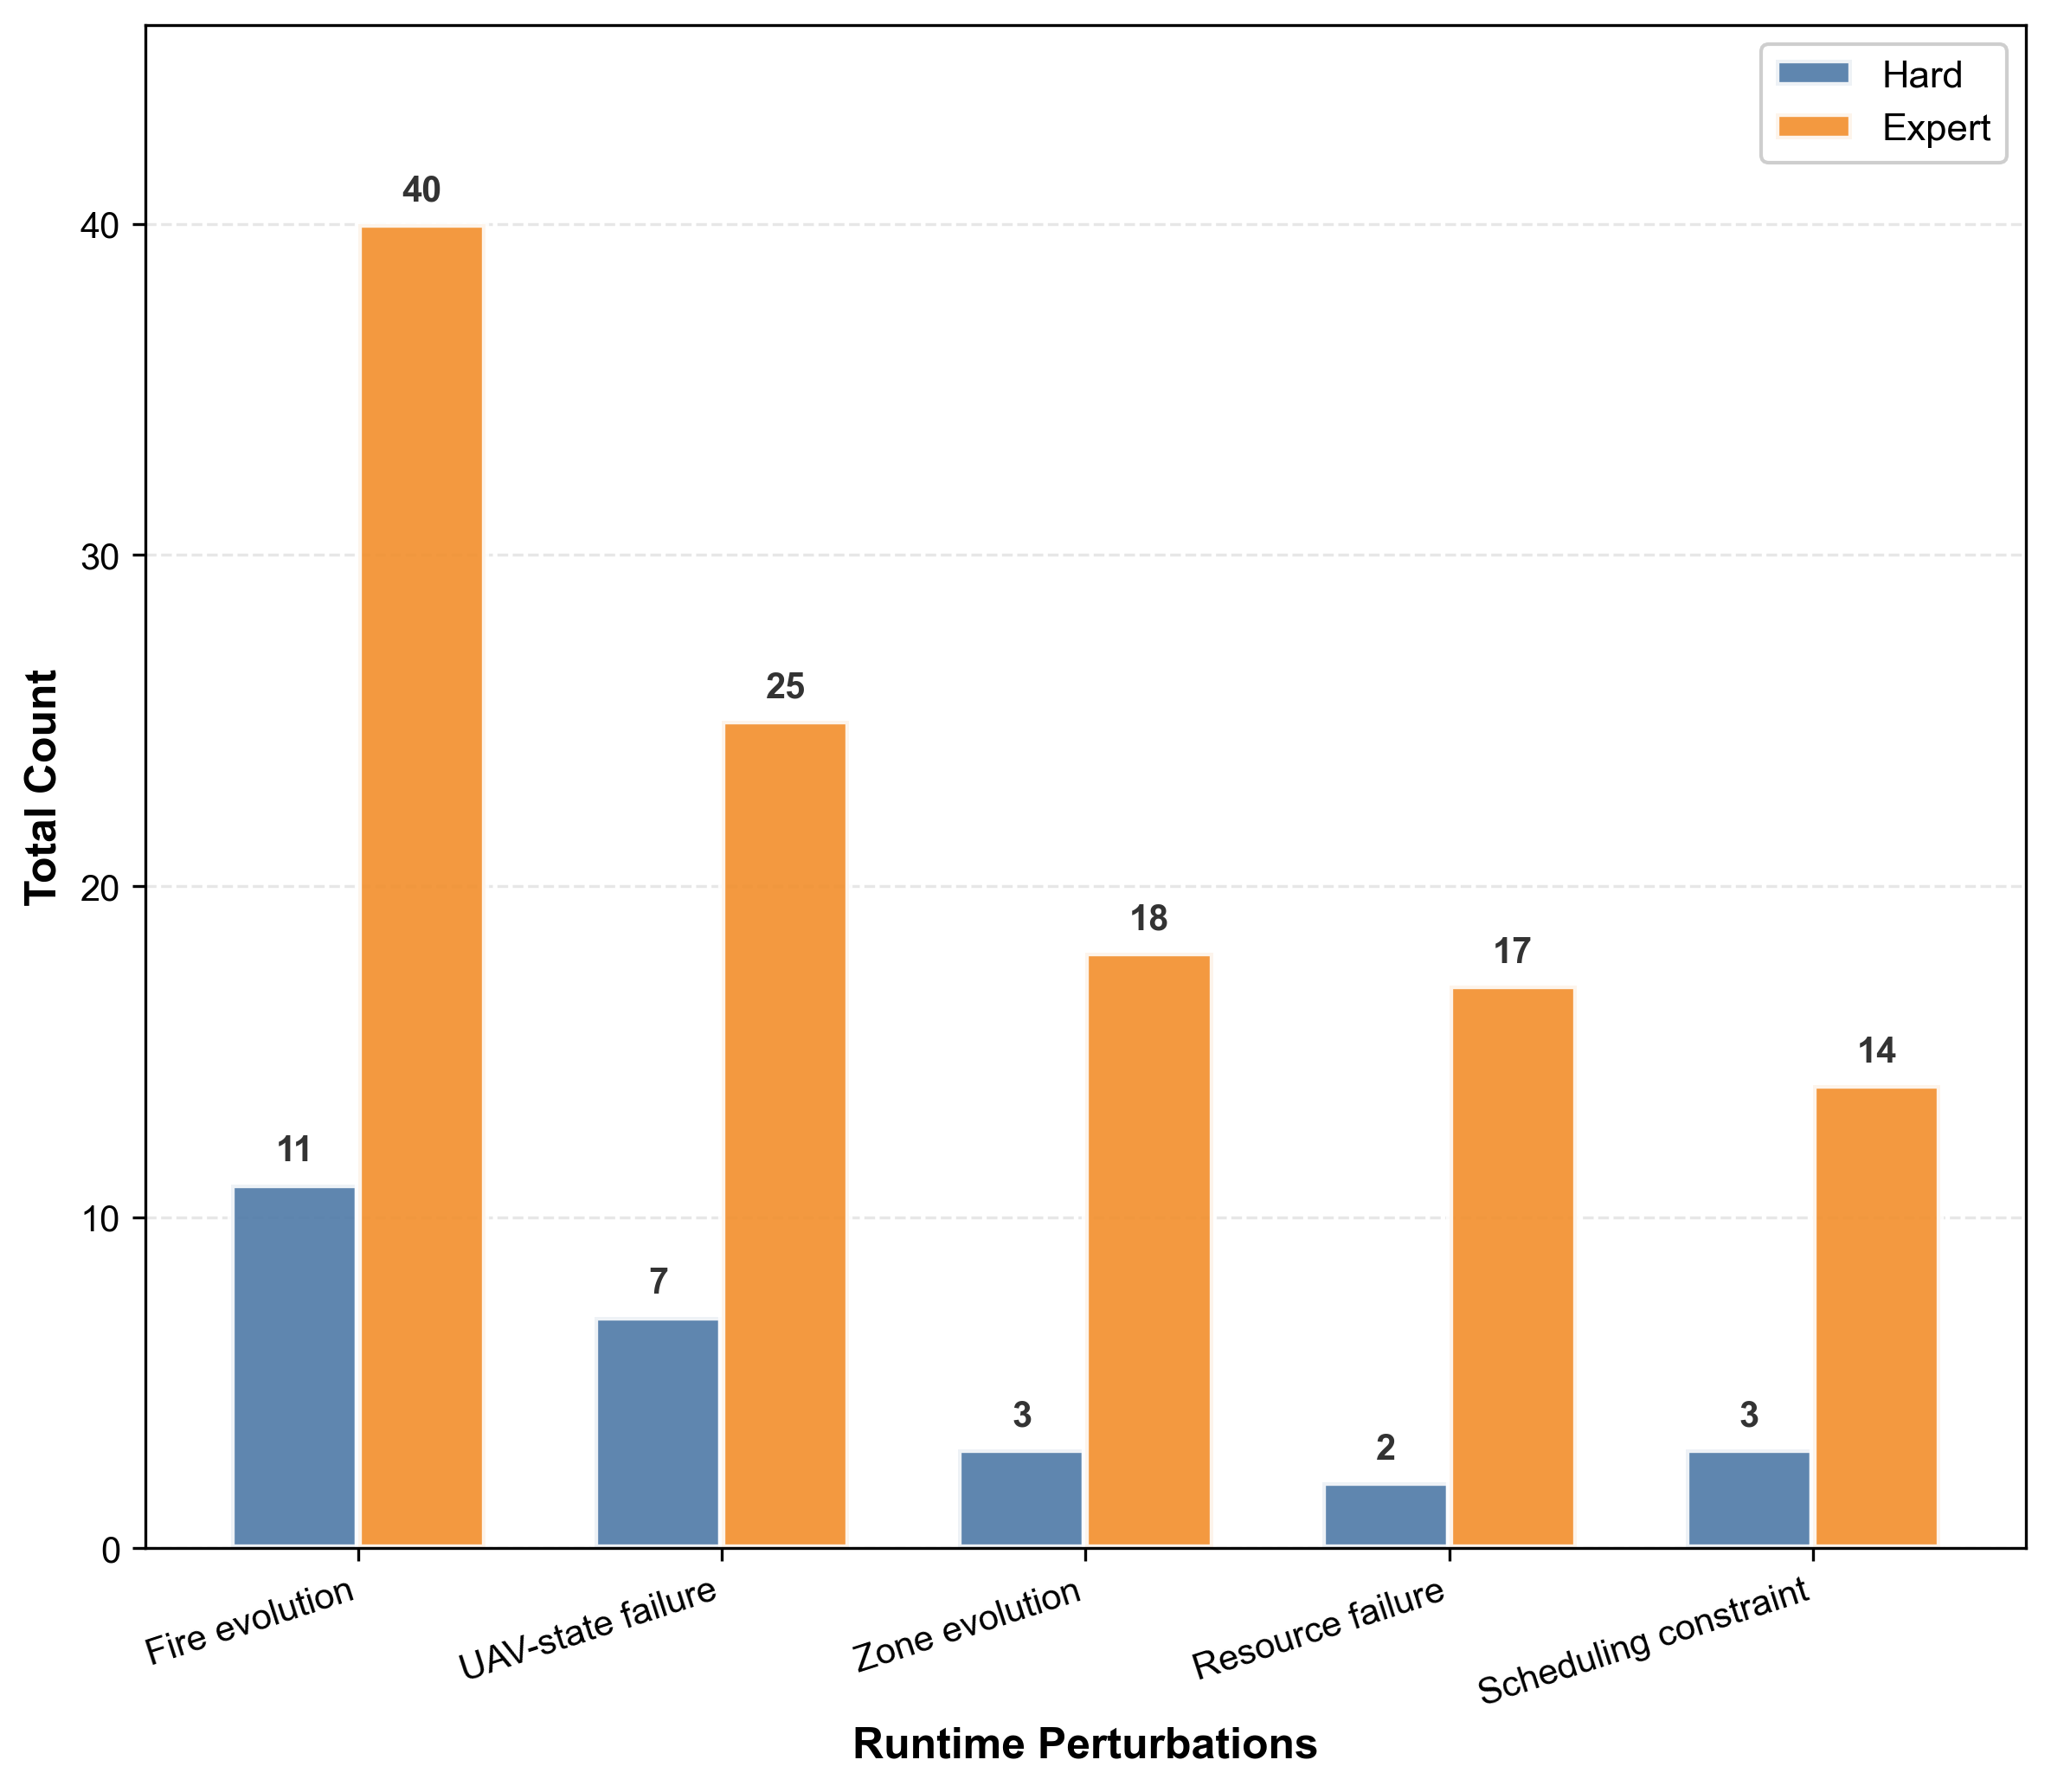
\includegraphics[width=0.485\textwidth]{figures/runtime-perturbation-sampling-distribution.png}}
    \caption{Runtime perturbations used for closed-loop evaluation.}
    \label{fig:runtime-perturbation-distribution}
\end{figure*}

\subsection{Evaluation Metrics}
We evaluate end-to-end behavior using six complementary mission-level metrics:
completion, response, mission time, event stability, resource pressure, and
coordination. They measure objective attainment, response timeliness, execution
efficiency, continuity under perturbations, resource use, and workload balance,
respectively. Event stability is evaluated only in the hard and expert settings,
where runtime perturbations are introduced.

All scores are normalized to $[0,100]$, with higher values indicating better
performance. Let $Z$ be the set of task zones, $c_z\in[0,1]$ the completion
ratio of zone $z$, and $\omega_z$ its priority weight. Let
$\bar t_{\mathrm{resp}}$ and $\tau$ denote the priority-weighted mean time to
first effective intervention and the total mission duration. The six scores are
defined jointly as
\begin{equation}
\begin{aligned}
s_{\mathrm{comp}}
&=100\frac{\sum_{z\in Z}\omega_zc_z}
 {\sum_{z\in Z}\omega_z},\\
s_{\mathrm{resp}}
&=100\left[1-
\left[\frac{\bar t_{\mathrm{resp}}-l_{\mathrm{resp}}}
 {u_{\mathrm{resp}}-l_{\mathrm{resp}}}\right]_0^1\right],\\
s_{\mathrm{time}}
&=100\left[1-
\left[\frac{\tau-l_{\mathrm{time}}}
 {u_{\mathrm{time}}-l_{\mathrm{time}}}\right]_0^1\right],\\
s_{\mathrm{stab}}
&=\frac{100}{N_e}\sum_{e=1}^{N_e}
 \mathbb{I}\bigl(\mathrm{Recovered}(e)\bigr),\\
s_{\mathrm{res}}
 &=100\left[1-\frac{\bar p+\max_jp_j}{2}\right],\\
s_{\mathrm{coord}}
&=100\left[1-
\frac{G(\mathbf{n})+G(\mathbf{d})+G(\boldsymbol{\tau})}{3}\right].
\end{aligned}
\label{eq:mission-level-scores}
\end{equation}
Here, $[x]_0^1=\min\{1,\max\{0,x\}\}$ clips a value to $[0,1]$;
$l_{\mathrm{resp}}$, $u_{\mathrm{resp}}$, $l_{\mathrm{time}}$, and
$u_{\mathrm{time}}$ are fixed time-reference thresholds. $N_e$ is the number
of runtime perturbations, and $\mathrm{Recovered}(e)$ indicates recovery by a
feasible revision within the allowed window. $p_j\in[0,1]$ and $\bar p$ denote
the per-UAV and fleet-average resource pressure. $G(\cdot)\in[0,1]$ is the
Gini coefficient of the assigned task counts $\mathbf{n}$, flight distances
$\mathbf{d}$, or execution durations $\boldsymbol{\tau}$.

Because no perturbations are introduced in the simple and normal settings,
their applicable metric set $\mathcal{K}_d$ contains completion, response,
mission time, resource pressure, and coordination; for the hard and expert
settings, it additionally contains event stability.
For each episode $i$ at difficulty level $d$, the score combines the weighted
aggregation of its applicable metrics with a bounded difficulty reward. The
reported score for level $d$ is the mean across its $N_d$ episodes:
\begin{equation}
\begin{aligned}
S_d
&=\frac{1}{N_d}\sum_{i=1}^{N_d}
\left[\sum_{k\in\mathcal{K}_d}w_{k,d}s_{i,k}
\frac{1+\lambda\rho_i}{1+\lambda}\right],\\
w_{k,d}&\geq0,\qquad
\sum_{k\in\mathcal{K}_d}w_{k,d}=1.
\end{aligned}
\label{eq:final-evaluation-score}
\end{equation}
where $w_{k,d}$ is the normalized weight of metric $k$ at difficulty level $d$,
$\rho_i\in[0,1]$ is the difficulty coefficient of episode $i$, and $\lambda\geq0$
controls the strength of the difficulty reward. The normalization by
$1+\lambda$ ensures that $S_d\in[0,100]$. The component scores remain
available for diagnostic analysis, while $S_d$ provides a unified measure for
overall comparison.

Together, the staged episode difficulty and decomposed metrics provide a common
basis for testing the three questions examined next: whether the complete
framework sustains high-level closed-loop decision making, which mechanisms
matter as operational pressure increases, and how much capability for
resource-constrained mission planning can be retained by a compact planner.

\endinput
